%%%%%%%%%%%%%%%%%%%%%%%%%%%%%%%%%%%%%%%%%%%%%%%%%%%%%%%%%%%%%%%%%%%%%%
% Problem statement
\begin{statement}[
  problempoints=110,
  timelimit=5 sekundi,
  memorylimit=512 MiB,
]{Lampice}

\setlength\intextsep{-0.1cm}
\begin{wrapfigure}[7]{r}{0.2\textwidth}
\centering
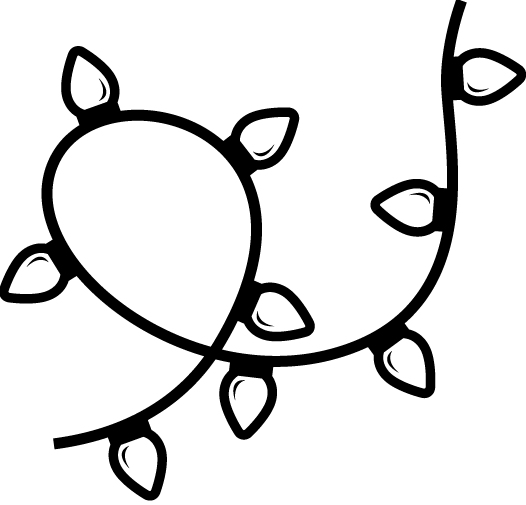
\includegraphics[width=0.2\textwidth]{img/lampice.png}
\end{wrapfigure}

Mirko je odabrao božićno drvce za nadolazeće blagdane te ga je odlučio ukrasiti
božićnim lampicama. Božićne lampice sastoje se od $N$ LED žaruljica povezanih s
$(N - 1)$ vodljivih žica tako da su sve žaruljice međusobno povezane. Dodatno,
za svaku žaruljicu poznata je boja kojom svijetli.

Nakon što je okitio drvce, Mirko se ponosno zagledao u svoje remek-djelo. Nakon
kraćeg gledanja, počeo je uočavati razne uzorke, među kojima su ga se posebno
dojmili tzv. \textit{palindromski segmenti}. Palindromski segment je dio na
božićnim lampicama između dvije žaruljice, $u$ i $v$, takav da je slijed boja na
putu od žaruljice $u$ do žaruljice $v$ jednak slijedu boja na putu od žaruljice
$v$ do žaruljice $u$.
Odredite duljinu najdužeg takvog segmenta, izraženu u broju žaruljica na tom
segmentu.

%Mirko želi pronaći najduži palindromski segment, ali žaruljica ima mnogo!
%Odredite duljinu najdužeg takvog segmenta, izraženu u broju žaruljica na tom
%segmentu.

%%%%%%%%%%%%%%%%%%%%%%%%%%%%%%%%%%%%%%%%%%%%%%%%%%%%%%%%%%%%%%%%%%%%%%
% Input
\subsection*{Ulazni podaci}
U prvom je retku prirodan broj $N$ $(1 \le N \le 50\ 000)$ iz teksta zadatka.

U sljedećem se retku nalazi niz od $N$ malih slova engleske abecede gdje $i$-to
slovo predstavlja boju kojom svijetli $i$-ta žaruljica.

U sljedećih se $(N - 1)$ redaka nalaze po dva broja $A$ i $B$
$(1 \le A, B \le N, A \neq B)$,
koja označavaju vodljivu žicu koja izravno povezuje žaruljice $A$ i $B$.

%%%%%%%%%%%%%%%%%%%%%%%%%%%%%%%%%%%%%%%%%%%%%%%%%%%%%%%%%%%%%%%%%%%%%%
% Output
\subsection*{Izlazni podaci}
U prvom i jedinom retku ispišite duljinu najdužeg palindromskog segmenta.

%%%%%%%%%%%%%%%%%%%%%%%%%%%%%%%%%%%%%%%%%%%%%%%%%%%%%%%%%%%%%%%%%%%%%%
% Scoring
 \subsection*{Bodovanje}
{\renewcommand{\arraystretch}{1.4}
  \setlength{\tabcolsep}{6pt}
  \begin{tabular}{ccl}
 Podzadatak & Broj bodova & Ograničenja \\ \midrule
  1 & 17 & $N \le 3000$ \\
  2 & 25 & \makecell[l]{
            % božićne lampice čine lanac, tj.
            Žaruljica $i$ je povezana sa žaruljicom
            $i+1$ $(1 \le i < N)$.
            } \\
  3 & 31 & Najviše $100$ lampica povezano je samo sa jednom drugom lampicom. \\
  4 & 37 & Nema dodatnih ograničenja. \\
\end{tabular}}

%%%%%%%%%%%%%%%%%%%%%%%%%%%%%%%%%%%%%%%%%%%%%%%%%%%%%%%%%%%%%%%%%%%%%%
% Examples
\subsection*{Probni primjeri}
\begin{tabularx}{\textwidth}{X'X'X}
\sampleinputs{test/lampice.dummy.in.1}{test/lampice.dummy.out.1} &
\sampleinputs{test/lampice.dummy.in.2}{test/lampice.dummy.out.2} &
\sampleinputs{test/lampice.dummy.in.3}{test/lampice.dummy.out.3}
\end{tabularx}

%%%%%%%%%%%%%%%%%%%%%%%%%%%%%%%%%%%%%%%%%%%%%%%%%%%%%%%%%%%%%%%%%%%%%%
% We're done
\end{statement}

%%% Local Variables:
%%% mode: latex
%%% mode: flyspell
%%% ispell-local-dictionary: "croatian"
%%% TeX-master: "../hio.tex"
%%% End:
